\documentclass[10pt]{article}
\usepackage[polish]{babel}
\usepackage[utf8]{inputenc}
\usepackage[T1]{fontenc}
\usepackage{amsmath}
\usepackage{amsfonts}
\usepackage{amssymb}
\usepackage[version=4]{mhchem}
\usepackage{stmaryrd}
\usepackage{graphicx}
\usepackage[export]{adjustbox}
\graphicspath{ {./images/} }

\title{PRACA KONTROLNA nr 7 - POZIOM PODSTAWOWY }

\author{}
\date{}


\begin{document}
\maketitle
\begin{enumerate}
  \item Liczba 1 jest pierwiastkiem wielomianu trzeciego stopnia $w(x)$ oraz wielomianu $w(x+1)$. Środkiem symetrii wykresu $w(x)$ jest punkt $S(0,2)$. Narysować staranny wykres funkcji $f(x)=|w(x-1)|$. (Środkiem symetrii krzywej o równaniu $y(x)=a x^{3}+b x^{2}+c x+d$ jest punkt $S\left(\frac{-b}{3 a}, y\left(\frac{-b}{3 a}\right)\right)$.)
  \item Sala jest oświetlona 5 żarówkami. Wkręcono losowo żarówki żółte, czerwone, zielone i niebieskie. Obliczyć prawdopodobieństwo, że wkręcono co najmniej dwie żarówki żółte i co najmniej dwie czerwone.
  \item Rozwiązać równanie
\end{enumerate}

$$
\frac{\cos 5 x}{\cos 3 x}+1=0
$$

\begin{enumerate}
  \setcounter{enumi}{3}
  \item Wazon w kształcie walca, którego wysokość jest większa od średnicy podstawy, ma objętość $1200 \mathrm{~cm}^{3}$. Napełniony wodą wazon przechylono tak, że jego oś symetrii utworzyła z pionem kạt $45^{\circ}$. Wylało się $200 \mathrm{~cm}^{3}$ wody. Podać wymiary wazonu (pominąć grubość ścianek).
  \item Podstawa $A B$ trapezu równoramiennego jest średnicą okręgu opisanego na nim. Za pomocą rachunku wektorowego wyznaczyć współrzędne wierzchołków $B$ i $C$, wiedząc, że $|A B|=5, A(1,1), D(3,2)$ oraz że $B$ leży w dolnej półpłaszczyźnie.
  \item Krzywa spiralna jest utworzona z ćwiartek okręoów, których promienie tworzą ciạg geo-\\
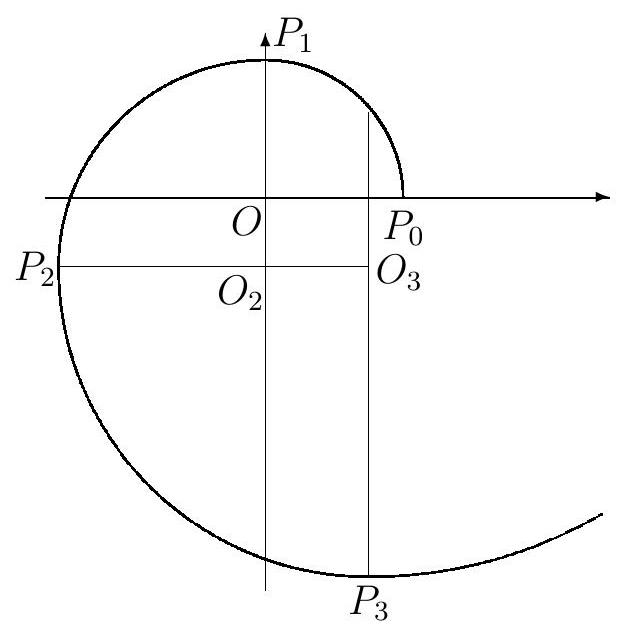
\includegraphics[max width=\textwidth, center]{2024_11_16_06775899c7f7a12bc0aag-1}\\
metryczny o ilorazie $q>1$. Środek pierwszego okręgu znajduje się w początku układu współrzędnych, a punkt $P_{0}(2,0)$ jest początkiem krzywej. Środek $O_{2}$ drugiego okręgu leży na osi Oy tak, że łuki obu okręgów łączą się w punkcie $P_{1}$ (rysunek). Środki kolejnych okręgón sa tak położone, że utworzona krzywa jest gładka i promień łuku mniejszego okręgu jest częścią promienia łuku większego okręgu (rysunek). Znaleźć współrzędne środka $O_{6}$ oraz długość łuku spirali $P_{0} P_{6}$. Wynik podać w najprostszej postaci. Następnie wykonać obliczenia dla $q=\frac{3}{2}$.
\end{enumerate}

\section*{PRACA KONTROLNA nr 7 - POZIOM ROZSZERZONY}
\begin{enumerate}
  \item Stosując zasadę indukcji matematycznej, wykazać, że dla wszystkich $n \geq 1$ liczba $10^{n}+18 n-1$ jest podzielna przez 27 .
  \item Sprawdzić tożsamość
\end{enumerate}

$$
\frac{\cos ^{2} \alpha-\cos ^{2} \beta}{\sin ^{2} \alpha-\cos ^{2} \beta}=\operatorname{tg}(\alpha+\beta) \operatorname{tg}(\alpha-\beta)
$$

i określić jej dziedzinę.\\
3. Dwóch strzelców oddało każdy po dwa strzały i okazało się, że cel został trafiony dokładnie dwa razy. Obliczyć prawdopodobieństwo, że dwukrotnie trafił pierwszy strzelec, jeśli za każdym razem pierwszy trafia z prawdopodobieństwem $\frac{4}{5}$, a drugi z prawdopodobieństwem $\frac{3}{5}$.\\
4. Znaleźć wartość parametru nieujemnego $p$, dla którego suma kwadratów odwrotności pierwiastków równania

$$
x^{2}+(p+1) x-(p+3)=0
$$

jest najmniejsza.\\
5. Rozwiązać układ równań

$$
\left\{\begin{array}{l}
x^{2} y^{2}=4 \\
y^{4}-6 y^{2}-x^{2}+9=0
\end{array}\right.
$$

Podać interpretację geometryczną tego układu i obliczyć pole wielokąta utworzonego przez jego rozwiązania (interpretowane jako punkty na płaszczyźnie). Sporządzić rysunek.\\
6. Podstawą ostrosłupa $A B C D$ jest trójkąt równoramienny o kącie przy wierzchołku $2 \alpha$. Płaszczyzna przechodząca przez wierzchołek $D$ ostrosłupa i wysokość podstawy jest płaszczyzną symetrii ostrosłupa, a przekrój bryły tą płaszczyzną jest trójkątem równobocznym o boku $a$. Wykazać, że ostrosłup ma jeszcze jedną płaszczyznę symetrii i obliczyć promień kuli opisanej na nim.

Rozwiązania (rękopis) zadań z wybranego poziomu prosimy nadsyłać do 18 marca 2018 r. na adres:

Wydział Matematyki\\
Politechniki Wrocławskiej,\\
ul. Wybrzeże Wyspiańskiego 27,\\
50-370 WROCŁAW.\\
Na kopercie prosimy koniecznie zaznaczyć wybrany poziom! (np. poziom podstawowy lub rozszerzony). Do rozwiązań należy dołączyć zaadresowaną do siebie kopertę zwrotną z naklejonym znaczkiem, odpowiednim do wagi listu. Prace nie spełniające podanych warunków nie będą poprawiane ani odsyłane.


\end{document}